\documentclass[solutionorbox,answers]{exam}

%%%%%%%%%%%%%%%%%%%%%%%%%%%%%%%%%%%%%%%%%%%%%%%%%%%%%%%%%%%%%%%
% Update to change header
\newcommand{\courseName}{CS 577}
\newcommand{\assignmentName}{Assignment 10 -- More Network Flow}
\newcommand{\semester}{Spring 2023}
%%%%%%%%%%%%%%%%%%%%%%%%%%%%%%%%%%%%%%%%%%%%%%%%%%%%%%%%%%%%%%%

\usepackage[utf8]{inputenc}
\usepackage[T1]{fontenc}

\usepackage{amsmath}
\usepackage{amsfonts}
\usepackage{amsthm}
\usepackage{booktabs}
\usepackage{listings}
\usepackage{tkz-graph}
\usepackage[ruled]{algorithm2e}
\usepackage{graphicx}

\usepackage{listings}
\lstset{basicstyle=\ttfamily,
  showstringspaces=false,
  commentstyle=\color{red},
  keywordstyle=\color{blue}
}

\usepackage{hyperref}

\pagestyle{headandfoot}
\runningheadrule
\firstpageheader{\courseName}{\huge \assignmentName}{\semester}
\runningheader{\courseName}
{\assignmentName}
{\semester}
\firstpagefooter{}{}{}
\runningfooter{}{Page \thepage\ of \numpages}{}

\begin{document}

\begin{center}
\fbox{\parbox{5.5in}{\centering
Answer the questions in the boxes provided on the
question sheets. If you run out of room for an answer,
add a page to the end of the document. \\
\vspace{0.1in}
}}
\end{center}
\vspace{0.1in}
\makebox[0.48\textwidth]{Name:\enspace\hrulefill} \qquad
\makebox[0.48\textwidth]{Wisc id:\enspace\hrulefill}

\section*{More Network Flow}

\begin{questions}
\question \textit{Kleinberg, Jon. Algorithm Design (p.416 q.6).}
Suppose you’re a consultant for the Ergonomic Architecture Commission,
and they come to you with the following problem.

They're really concerned about designing houses that are ``user-friendly'', and they've been having a lot of trouble with the setup of light
fixtures and switches in newly designed houses. Consider, for example,
a one-floor house with $n$ light fixtures and $n$ locations for light switches
mounted in the wall. You'd like to be able to wire up one switch to control
each light fixture, in such a way that a person at the switch can see the
light fixture being controlled.

\begin{figure}[h]
  \centering
  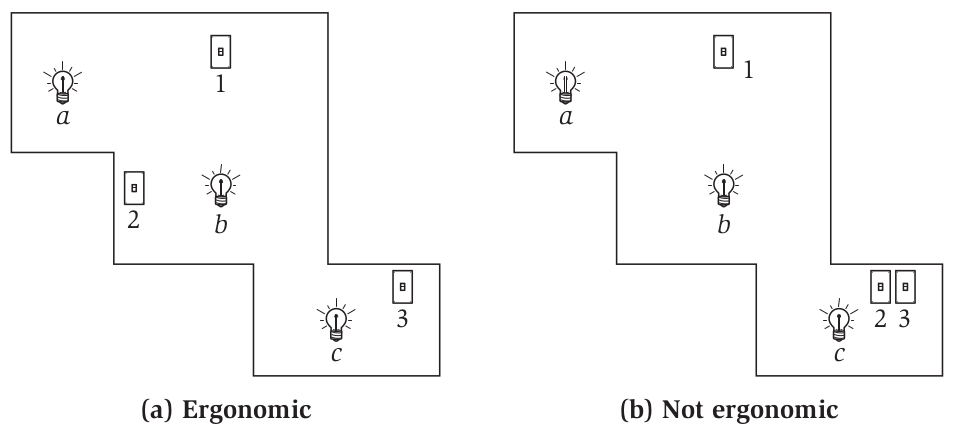
\includegraphics[width=\textwidth]{fig728.png}
  \caption{The floor plan in (a) is ergonomic, because we can wire switches to fixtures
in such a way that each fixture is visible from the switch that controls it. (This can be
done by wiring switch 1 to a, switch 2 to b, and switch 3 to c.) The floor plan in (b) is not
ergonomic, because no such wiring is possible.}
\end{figure}

Sometimes this is possible and sometimes it isn't. Consider the two
simple floor plans for houses in Figure 1. There are three light fixtures
(labelled $a, b, c$) and three switches (labelled 1, 2, 3). It is possible to wire switches to fixtures in Figure 1(a) so that every switch has a line of
sight to the fixture, but this is not possible in Figure 1(b).

Let's call a floor plan, together with $n$ light fixture locations and $n$
switch locations, ergonomic if it's possible to wire one switch to each
fixture so that every fixture is visible from the switch that controls it.
A floor plan will be represented by a set of $m$ horizontal or vertical
line segments in the plane (the walls), where the $i$-th wall has endpoints
$(x_i, y_i), (x'_i, y'_i)$. Each of the $n$ switches and each of the $n$ fixtures is given by its coordinates in the plane. A fixture is visible from a switch if the line segment joining them does not cross any of the walls.

Give an algorithm to decide if a given floor plan is ergonomic. The
running time should be polynomial in $m$ and $n$. You may assume that you
have a subroutine with $O(1)$ running time that takes two line segments as input and decides whether or not they cross in the plane.

\newpage

\begin{solutionbox}{\stretch{1}} \\

\end{solutionbox}

\newpage

\question \textit{Kleinberg, Jon. Algorithm Design (p.426 q.20).}

Your friends are involved in a large-scale atmospheric science experiment. They need to get good measurements on a set $S$ of $n$ different
conditions in the atmosphere (such as the ozone level at various places),
and they have a set of $m$ balloons that they plan to send up to make these
measurements. Each balloon can make at most two measurements.
Unfortunately, not all balloons are capable of measuring all conditions, so for each balloon $i = 1,\ldots,m$, they have a set $S_i$ of conditions
that balloon $i$ can measure. Finally, to make the results more reliable, they
plan to take each measurement from at least $k$ different balloons. (Note
that a single balloon should not measure the same condition twice.) They
are having trouble figuring out which conditions to measure on which
balloon.

\paragraph{Example.} Suppose that $k = 2$, there are $n = 4$ conditions labelled $c_1,c_2,c_3,c_4$,
and there are $m = 4$ balloons that can measure conditions, subject to
the limitation that $S_1 = S_2 = {c_1,c_2,c_3}$, and $S_3 = S_4 = {c_1,c_3,c_4}$. Then one possible way to make sure that each condition is measured at least $k = 2$ times is to have
\begin{itemize}
\item balloon 1 measure conditions $c_1, c_2$,
\item balloon 2 measure conditions $c_2, c_3$,
\item balloon 3 measure conditions $c_3, c_4$, and
\item balloon 4 measure conditions $c_1, c_4$.
\end{itemize}

\begin{parts}
  \part Give a polynomial-time algorithm that takes the input to an instance
of this problem (the $n$ conditions, the sets $S_i$ for each of the $m$
balloons, and the parameter $k$) and decides whether there is a way to
measure each condition by $k$ different balloons, while each balloon
only measures at most two conditions.

\begin{solutionbox}{\stretch{1}} \\

\end{solutionbox}

\newpage

\part You show your friends a solution computed by your algorithm from
(a), and to your surprise they reply, ``This won't do at all—one of the
conditions is only being measured by balloons from a single subcontractor.'' You hadn't heard anything about subcontractors before; it
turns out there's an extra wrinkle they forgot to mention...

Each of the balloons is produced by one of three different subcontractors involved in the experiment. A requirement of the experiment is that there be no condition for which all $k$ measurements come from balloons produced by a single subcontractor.

Explain how to modify your polynomial-time algorithm for part
(a) into a new algorithm that decides whether there exists a solution
satisfying all the conditions from (a), plus the new requirement about
subcontractors.

\begin{solutionbox}{\stretch{1}} \\

\end{solutionbox}

\end{parts}

\newpage

\question \textit{Kleinberg, Jon. Algorithm Design (p.442, q.41).} 

Suppose you're managing a collection of $k$ processors and must schedule a sequence of $m$ jobs over $n$ time steps.

The jobs have the following characteristics. Each job $j$ has an arrival
time $a_j$ when it is first available for processing, a length $\ell_j$ which indicates
how much processing time it needs, and a deadline $d_j$ by which it must
be finished. (We'll assume $0 < \ell_j \le d_j - a_j$.) Each job can be run on any
of the processors, but only on one at a time; it can also be preempted
and resumed from where it left off (possibly after a delay) on another
processor.

Moreover, the collection of processors is not entirely static either:
You have an overall pool of $k$ possible processors; but for each processor
$i$, there is an interval of time $[t_i , t'_i]$ during which it is available; it is
unavailable at all other times.

Given all this data about job requirements and processor availability,
you'd like to decide whether the jobs can all be completed or not. Give a
polynomial-time (in $k$, $m$, and $n$) algorithm that either produces a schedule completing all
jobs by their deadlines or reports (correctly) that no such schedule exists.
You may assume that all the parameters associated with the problem are
integers.
{\small
\paragraph{Example.} Suppose we have two jobs $J_1$ and $J_2$. $J_1$ arrives at time 0, is due
at time 4, and has length 3. $J_2$ arrives at time 1, is due at time 3, and has
length 2. We also have two processors $P_1$ and $P_2$. $P_1$ is available between
times 0 and 4; $P_2$ is available between times 2 and 3. In this case, there is
a schedule that gets both jobs done.
\begin{itemize}
\item At time 0, we start job $J_1$ on processor $P_1$.
\item At time 1, we preempt $J_1$ to start $J_2$ on $P_1$.
\item At time 2, we resume $J_1$ on $P_2$. ($J_2$ continues processing on $P_1$.)
\item At time 3, $J_2$ completes by its deadline. $P_2$ ceases to be available, so
we move $J_1$ back to $P_1$ to finish its remaining one unit of processing
there.
\item At time 4, $J_1$ completes its processing on $P_1$.
Notice that there is no solution that does not involve preemption and
moving of jobs.
\end{itemize}
}
\begin{solutionbox}{\stretch{1}}

\end{solutionbox}

\newpage

\question \textit{Kleinberg, Jon. Algorithm Design (p.444, q.45).} 

Consider the following definition. We are given a set of $n$ countries that are engaged in trade with one another. For each country $i$, we have the value $s_i$ of its budget surplus; this number may be positive or negative,
with a negative number indicating a deficit. For each pair of countries $i, j$,
we have the total value $e_{ij}$ of all exports from $i$ to $j$; this number is always
nonnegative. We say that a subset $S$ of the countries is \emph{free-standing} if the
sum of the budget surpluses of the countries in $S$, minus the total value
of all exports from countries in $S$ to countries not in $S$, is nonnegative.
Give a polynomial-time algorithm that takes this data for a set of
$n$ countries and decides whether it contains a nonempty free-standing
subset that is not equal to the full set.

\begin{solutionbox}{\stretch{1}}

\end{solutionbox}

\newpage

\question

Implement an algorithm to determine the maximum matching in a bipartite graph and if that matching is perfect (all nodes are matched) in either C, C++, C\#, Java, Python, or Rust. Be efficient and use your max-flow implementation from the previous week. 

The input will start with an positive integer, giving the number of instances that follow. For each instance, there will be 3 positive integers $m$, $n$, and $q$. Numbers $m$ and $n$ are the number of nodes in node set $A$ and node set $B$. Number $q$ is the number of edges in the bipartite graph. For each edge, there will be 2 more positive integers $i$, and $j$ representing an edge between node $1 \le i \le m$ in $A$ and node $1 \le i \le n$ in $B$. 

A sample input is the following:
\begin{verbatim}
3
2 2 4
1 1
1 2
2 1
2 2
2 3 4
2 3
2 1
1 2
2 2
5 5 10
1 1
1 3
2 1
2 2
2 3
2 4
3 4
4 4
5 4
5 5
\end{verbatim}
The sample input has 3 instances.

For each instance, your program should output the size of the maximum matching, followed by a space, followed by an $N$ if the matching is not perfect and a $Y$ if the matching is perfect. Each output line should be terminated by a newline. The correct output to the sample input would be:
\begin{verbatim}
2 Y
2 N
4 N
\end{verbatim}

\end{questions}

\end{document}